\subsection{Анализ с использованием нейронных сетей}
\label{sec:experiment:neural_engines}

Для сравнения также было решено разработать методику оценки стоимости недвижимости с использованием
нейронных сетей. Задача оценки недвижимости схематично представлена на рисунке~\ref{fig:experiment:neural-scheme}

\begin{figure}[!ht]
  \centering
  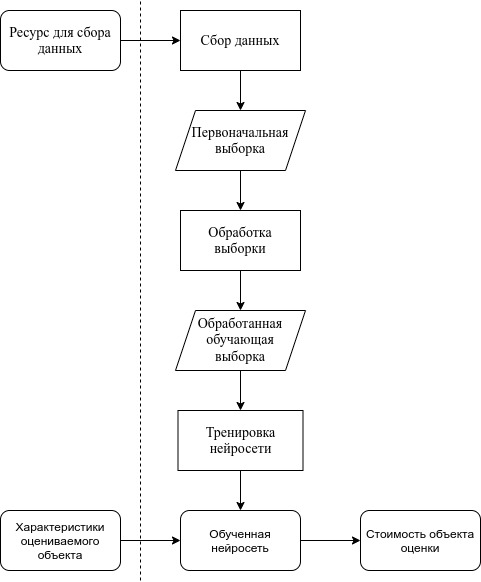
\includegraphics[scale=0.8]{neural-scheme.jpg} 
  \caption{Cхема использования нейронных сетей для оценки стоимости недвижимости}
  \label{fig:experiment:neural-scheme}
\end{figure}

Для достижения цели необходимо выбрать факторы, влияющие на	рыночную стоимость объектов недвижимости, подготовить выборку для
обучения нейронной сети. Обучающая выборка построена для проектирования и обучения нейронной сети с учителем,
поскольку такой тип нейронных сетей больше всего подходит для задач, когда имеется большой набор настоящих данных для обучения
алгоритма. Исходя из сравнительного анализа нескольких типов нейронных сетей с учителем, проведенного в статье, было
решено использовать нейронную сеть многослойный персептрон c использованием метода обратного распространения ошибки.
Многослойным персептроном называют нейронную сеть прямого распространения, где входной сигнал распространяется от слоя
к слою в прямом направлении. В общем представлении такая нейронная сеть состоит из:
\begin{itemize}
  \item множества входных узлов, образующих входной слой;
  \item одного или нескольких скрытых слоев вычислительных нейронов;
  \item одного выходного слоя нейронов.
\end{itemize}

Обощенная схема многослойного персептрона показана на рисунке~\ref{fig:experiment:perceptron-scheme}
\begin{figure}[!ht]
  \centering
  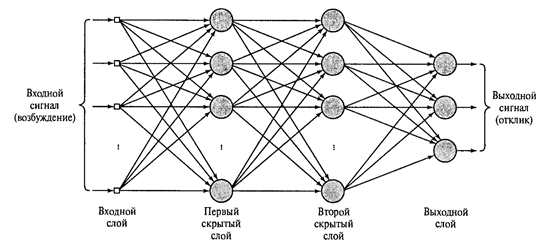
\includegraphics[scale=2]{perceptron.png}
  \caption{Cхема многослойного персептрона}
  \label{fig:experiment:perceptron-scheme}
\end{figure}

В качестве инструментального средства проектирования нейронной сети была выбрана STATISTICA Neural Networks.
Для обучения многослойных персептронов в пакете STATISTICA Нейронные сети реализовано пять различных алгоритмов
обучения. Это хорошо известный алгоритм обратного распространения, быстрые методы второго порядка – спуск по сопряженным
градиентам и Левенберга–Маркара, а также методы быстрого распространения и «дельта–дельта с чертой» (представляющие
собой вариации метода обратного распространения, которые в некоторых случаях работают быстрее).

Алгоритм обратного распространения ошибки является популярным алгоритмом обучения нейронных сетей с учителем. В основе
идеи алгоритма лежит использование выходной ошибки нейронной сети для вычисления величин коррекции весов нейронов в скрытых слоях

\begin{equation}
  E = \frac{1}{2}\sum_{i=1}^{k}\left(y-y'\right)^2
\end{equation}

\begin{explanation}
  где & $ k $ & число выходных нейронов сети,\\
  & $ y $ & целевое значение, \\
  & $ y' $ & фактическое выходное значение.\\ 
\end{explanation}

Алгоритм является итеративным. На каждой итерации происходит прямой и обратный проходы. На прямом проходе входной вектор распространяется
входов сети к ее выходам, в результате формируется выходной вектор, который соответствует фактическому состоянию весов.
После вычисляется ошибка нейронной сети как разность между фактическим и целевым значениями.
На обратном проходе эта ошибка распространяется от выхода сети к ее входам, и производится коррекция весов нейронов.
Полученные данные дают возможность с достаточной точностью прогнозировать стоимость объектов недвижимости по заданным параметрам.

Реализованные алгоритмы обучения представлены на рисунке~\ref{fig:experiment:network_configs}.\linebreak Кроме того, можно
заметить, что в зависимости от алгоритма обучения и выбранной функции активации изменялась и конфигрурация многослойного
персептрона. Так, самой эффективной оказалась конфигурация с 21 нейроном на первом скрытом слое, на втором – 9. На
обучение отводилось 4000 объектов из обучающей выборки, что составляет 70\% от общего числа объектов,
на контроль и тестирование по 15\% - по 600 объектов. Обучение производится по методу обратного распространения ошибки.

\begin{figure}[!ht]
  \centering
  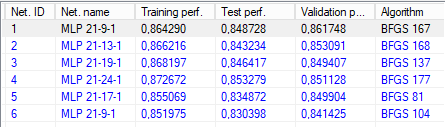
\includegraphics[scale=1.2]{network_configs.png}
  \caption{Параметры качества реализованных алгоритмов обучения}
  \label{fig:experiment:network_configs}
\end{figure}

Сравнение результатов ожидаемых с полученными представлено на рисунке~\ref{fig:experiment:neural_results}.
В первом столбце указана ожидаемая стоимость, во втором - полученная, в третьем - величина ошибки.
Как можно заметить ошибка варьируется и может составлять как и небольшие значения так и значительные.
Соотношение ожидаемых результатов с полученными показаны в виде графика на рисунке~\ref{fig:experiment:target_vs_output_neural}.

\begin{figure}[!ht]
  \centering
  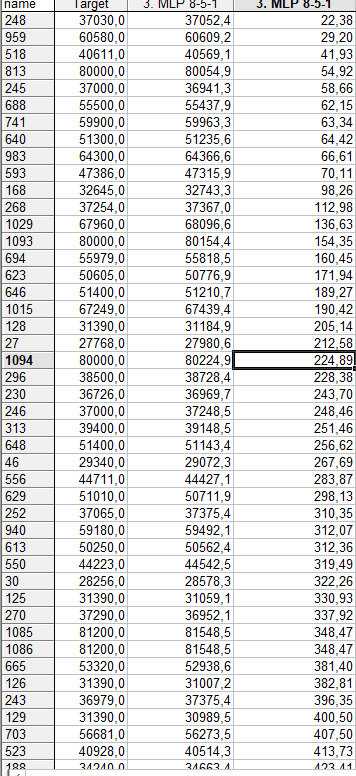
\includegraphics[scale=1]{neural_results.png}
  \caption{Сравнение полученных результатов с ожидаемыми}
  \label{fig:experiment:neural_results}
\end{figure}

\begin{sidewaysfigure}
  \centering
  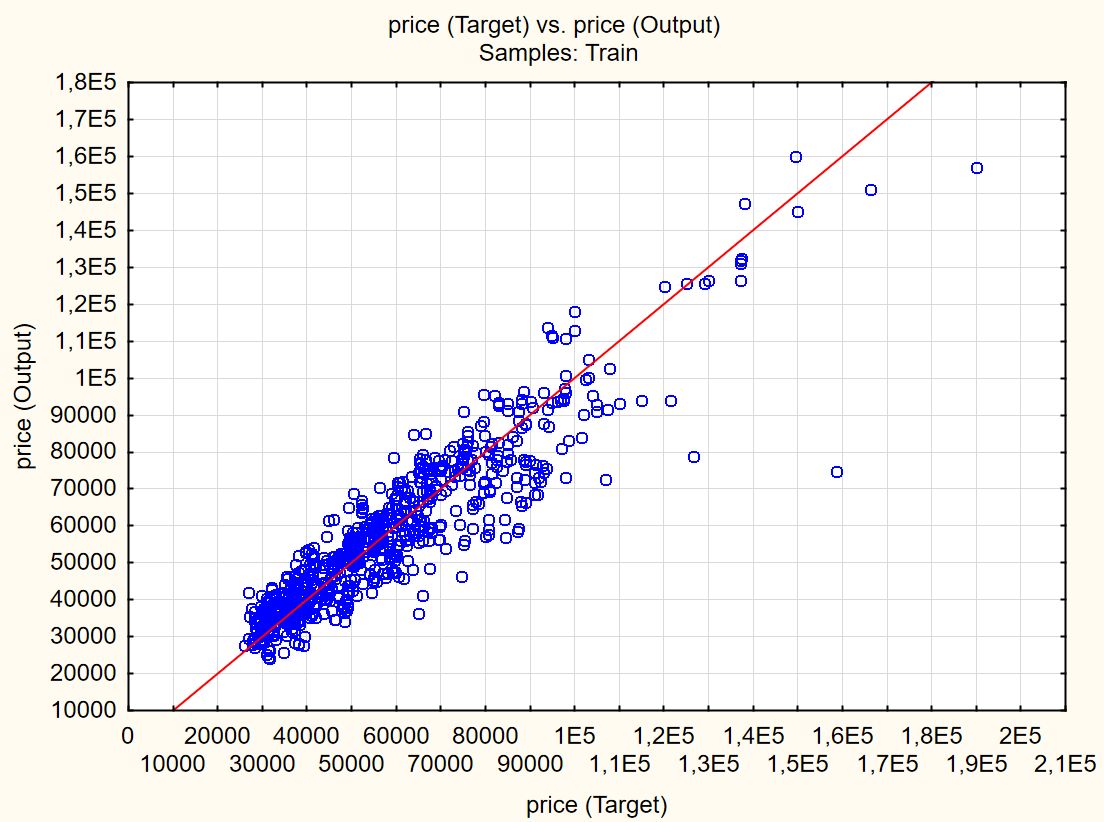
\includegraphics[scale=0.7]{target_vs_output_neural.png}
  \caption{Соотношение полученных результатов с ожидаемыми}
  \label{fig:experiment:target_vs_output_neural}
\end{sidewaysfigure}


